\documentclass[a4paper,14pt]{extarticle} % the default article class is limited to 12pt, but you can go up to 14, 17 or 20 points if you use the extarticle class
\usepackage{cmap} % make LaTeX PDF output copy-and-pasteable
\usepackage[T2A]{fontenc}
\usepackage[utf8]{inputenc}
\usepackage[english,ukrainian]{babel}

\usepackage{amssymb,amsfonts,mathtools,amsmath,cite,enumerate,float}
\usepackage{indentfirst} % set an additional space before a paragraph at the begining of new section
\usepackage{setspace}
\usepackage{textcomp}

\usepackage{leftidx} % this package enables left subscripts and superscripts in math mode.

\usepackage{import} % for adding a file by path https://tex.stackexchange.com/questions/246/when-should-i-use-input-vs-include

\usepackage{geometry} 
\geometry{left=1.25cm}
\geometry{right=1.25cm}
\geometry{top=1cm}
\geometry{bottom=2cm}

\usepackage[table,xcdraw,dvipsnames]{xcolor}
\usepackage{color}
% 1) tutorial about xcolor:  https://www.overleaf.com/learn/latex/Using_colours_in_LaTeX
% 2) huge tutorial about xcolor: https://latex-tutorial.com/color-latex/ 
% 3) RGB calculator: https://www.w3schools.com/colors/colors_rgb.asp

\usepackage{hyperref}
\definecolor{linkcolor}{HTML}{0000FF}
\definecolor{urlcolor}{HTML}{0000FF} 
\hypersetup{pdfstartview=FitH, unicode=true, linkcolor=linkcolor, urlcolor=urlcolor, colorlinks=true}

\usepackage{graphicx}
\usepackage{wrapfig}
\graphicspath{{Images/}} % path to images

\parskip=1mm % space between paragraphs

\usepackage{listingsutf8} % origin: \usepackage{listings}

\lstset{
    frame=single, %lines
    language=Python,
    aboveskip=3mm,
    belowskip=3mm,
    columns=flexible,
    basicstyle={\small\ttfamily},
    numbers=left,
    numberstyle=\tiny\color{gray},
    commentstyle=\color{OliveGreen},
    stringstyle=\color{Mahogany},
    morestring=[b]''',
    showstringspaces=false,
    keywordstyle=\bfseries\color{blue},
    emph={[1]import, as, for, return}, emphstyle={[1]\bfseries\color{magenta}},
    emph={[2]range}, emphstyle={[2]\bfseries\color{brown}},
    breaklines=true,
    breakatwhitespace=true,
    tabsize=4,
    extendedchars=false, % to use ukrainian text in a code
    inputencoding=utf8 % to use ukrainian text in a code
}

\begin{document}

\import{Title/}{title}

\newpage
\subsection*{Завдання}

Методами Рунге-Кутта четвертого порядку та Адамса-Башфорта четвертого порядку розв'язати задачу Коші. На
початку інтервалу у необхідній кількості точок значення для методу  Адамса-Башфорта визначити методом
Рунге-Кутта четвертого порядку.

\subsection*{Варіант завдання}

Рівняння має вигляд: 
\begin{equation}
    \frac{dy}{dt}=(1-x^2)y + F(x) \label{formula: initial equation}
\end{equation}

Покладемо крок $h=0.1$. Нехай розв'язок відомий та визначається згідно варіанту так: $y=\tg x$. 
Знаючи точний розв'язок, визначимо початкові умови: при $x_0=0$ значення $y_0(x_0)=\tg x_0=0$. 
Аналогічним чином довизначимо доданок $F(x)$, підставивиши точний розв'язок у рівняння 
(\ref{formula: initial equation}). Остаточно отримаємо: 
\begin{equation}
    \frac{dy}{dt}=f(x,y),\ \text{де}\ f(x,y)=(1-x^2)(y-\frac{\sin x}{\cos x}) + \frac{1}{\cos^2 x} \label{formula: first equation}
\end{equation}

\subsection*{Теоретичні відомості}

\subsubsection*{Метод Рунге-Кутта}

Числове розв'язання задачі полягає у побудові деякої таблиці наближених значень $y_1, y_2, \ldots, y_n$
розв'язку $y(x)$ у заданих точках $x_1, x_2, \ldots, x_n$. Метод Рунге-Кутта відносять до однокрокових методів, 
тобто таких, які використовують для наближеного обчислення поточного значення лише попередні елементи. 
На практиці найчастіше використовують формули метода Рунге-Кутта четвертого порядку (наявні чотири коефіцієнти). 
Вони мають такий вигляд:
\begin{align*}
    &y_{i+1}=y_i + \tfrac{1}{6}(k_1 + 2k_2 + 2k_3 + k_4) \\ \\
    &\begin{cases}
        k_1=hf(x_i,y_i) \\
        k_2=hf(x_i+0.5h,y_i+0.5k_1) \\
        k_3=hf(x_i+0.5h,y_i+0.5k_2) \\
        k_4=hf(x_i+h,y_i+k_3)
    \end{cases}
\end{align*} 

\subsubsection*{Метод Адамса-Башфорта}

Суть методу аналогічна до попереднього, проте метод Адамса-Башфорта відносять до багатокрокового, а отже, 
для наближеного обчислення поточного значення будуть використовуватися й попередні елементи (наприклад, для 
для методу четверного порядку -- попередні чотири значення):
\[ y_{i+1}=y_i + h(55f(x_i,y_i) - 59f(x_{i-1},y_{i-1}) + 37f(x_{i-2},y_{i-2}) -  9f(x_{i-3},y_{i-3})) \]

Відповідно, перші декілька значень $y_i$ знайдемо за методом Рунге-Кутта, а вже далі матимемо можливість 
запустити й метод Адамса-Башфорта.

\subsection*{Програмний код та проміжні результати}

\subsubsection*{Програмний код методів наближеного обчислення}

\lstinputlisting{Code/Runge_Kutta and Adams_Bashforth.py}

\begin{figure}[H]
    \center{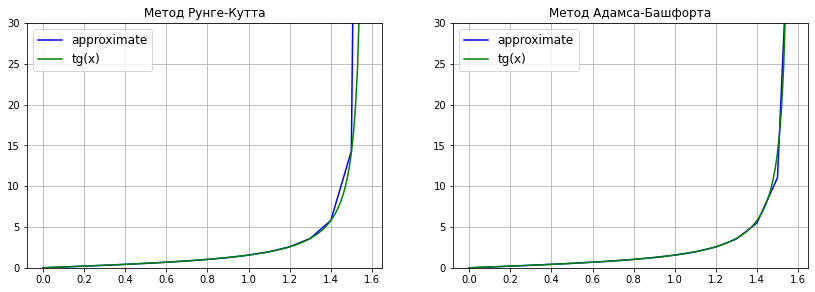
\includegraphics[width=1\linewidth]{R&A.png}}
    \caption{Результати наближених обчислень}
    \label{fig:R&A}
\end{figure}

\subsubsection*{Порівняльний аналіз похибок}

\lstinputlisting{Code/Error.py}

\begin{figure}[H]
    \center{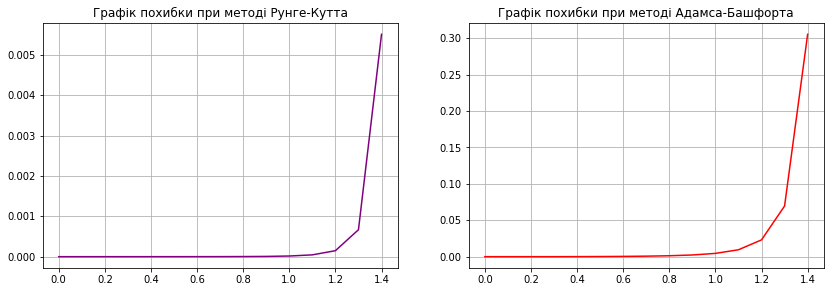
\includegraphics[width=1\linewidth]{R&A_errors.png}}
    \caption{Графіки похибок обчислень}
    \label{fig:Errors}
\end{figure}

\subsection*{Контрольні запитання}

\begin{enumerate}
    \item \textit{Яким чином визначають початкові точки для методів Адамса?}

    Спершу для визначення початкових точок використовують однокрокові методи (наприклад, у цій 
    лабораторній роботі було використано метод Рунге-Кутта). А далі -- настає етап власне 
    багатокрокових методів Адамса.
    
    \item \textit{Що таке однокрокові та багатокрокові методи розв’язання звичайних диференційних
    рівнянь?}
    
    До однокрокових відносять методи, які використовують для наближеного обчислення поточного значення лише 
    і тільки елементи з одного попереднього кроку. Натомість багатокрокові схеми -- залежно від порядку -- 
    для аналогічної задачі використовують певну кількість елементів із декількох попередніх кроків.  
    
\end{enumerate}

\end{document}